\documentclass[a4paper, table]{article}

\usepackage{xcolor}
\usepackage{amssymb}
\usepackage[a4paper]{geometry}
\usepackage[T1]{fontenc}
\usepackage[utf8]{inputenc}
\usepackage{graphicx}
\graphicspath{ {images/} }
\usepackage{todonotes}
\usepackage{hyperref}
\usepackage{longtable}
\hypersetup{
    colorlinks=true,
    linkcolor=black,
    filecolor=magenta,
    urlcolor=blue
}
% changes font
\usepackage[style=verbose-ibid,backend=bibtex]{biblatex}
\bibliography{wipro-main-doc}

\newcommand{\tabitem}{~~\llap{\textbullet}~~}

\usepackage{times}

% Set name of image label
\renewcommand{\figurename}{Abbildung}

\title{
    {Wirtschaftsprojekt} \\
    \vspace{10mm}
    { Herbstsemester 2022 } \\
    \vspace{10mm}
    % https://commons.wikimedia.org/wiki/File:HSLU_2022_logo.svg
    {
\includegraphics[width=75mm]{img/hsluLogo2022.png}}
}

\author{Yannis Kr\"amer und Nicolas Wiedmer}
% TODO: Update date
\date{22.09.2022}

\begin{document}

\maketitle

\newpage

\noindent
\fontsize{12}{14}
\textbf{Wirtschaftsprojekt an der Hochschule Luzern -- Informatik} \\ \vspace*{0.6cm}

\fontsize{10.95}{12}
\noindent
\textbf{Titel:} STAIR Discord Bot \\ \vspace*{0.2cm}

\noindent
\textbf{Studentin/Student:} Yannis Kr\"amer \newline \newline
\textbf{Studentin/Student:} Nicolas Wiedmer \newline \newline
\textbf{Studiengang:} BSc Informatik oder Wirtschaftsinformatik  \newline \newline
\textbf{Jahr:} 2022 \newline \newline
\textbf{Betreuungsperson:} Markus Waldmann \newline \newline
\textbf{Expertin/Experte:} \newline \newline
\textbf{Auftraggeberin/Auftraggeber:} STAIR (Martin Steiger \& Estefania Otero)\newline \newline \newline
\textbf{Codierung / Klassifizierung der Arbeit:}\\
$\boxtimes$ \"Offentlich
$\square$ Vertraulich


%%% you can use \boxtimes for filling a cross inside the square
%%% e.g., $\boxtimes$ A: Einsicht 	(Normalfall)


\paragraph{\textbf{Eidesstattliche Erkl\"arung}}
Ich erkl\"are hiermit, dass ich/wir die vorliegende Arbeit selbst\"andig und ohne unerlaubte fremde Hilfe angefertigt haben, alle verwendeten Quellen, Literatur und andere Hilfsmittel angegeben haben, w\"ortlich oder inhaltlich entnommene Stellen als solche kenntlich gemacht haben, das Vertraulichkeitsinteresse des Auftraggebers wahren und die Urheberrechtsbestimmungen der Hochschule Luzern respektieren werden. \newline \newline
Ort / Datum, Unterschrift	\underline{\hspace*{8cm}} \newline \newline
Ort / Datum, Unterschrift	\underline{\hspace*{8cm}} \newline \newline \newline
\textbf{Ausschliesslich bei Abgabe in gedruckter Form: \\
Eingangsvisum durch das Sekretariat auszuf\"ullen}\newline \newline
Rotkreuz, den	\underline{\hspace*{4cm}}	\hspace*{1cm} Visum:	\underline{\hspace*{4cm}}

\newpage
\section*{I{\hspace*{1cm}}Abstract}
\todo{schreiben}

\newpage

\tableofcontents

\newpage

\section{Problem, Fragestellung, Vision}
Die bisherige Lösung ist instabil und führt regelmässig zu Problemen.
So zum Beispiel funktionieren gewisse Befehle von Nadeko nicht mehr.
Was dazu geführt hat ist nicht bekannt.
Der Stan-Bot hat keine Bugs, jedoch gibt es hin und wieder unklarheiten bei den Studenten,
weshalb diese nachfragen in den Hilf-Channels auf dem Discord Server.
In der neuen Version sollten die nächsten Schritte und Abläufe für die Studenten verdeutlicht werden.
\newline
Die Lösung soll vereinheitlicht werden, was langzeitig Zeit bei der Übergabe an die nächsten Vorstandsmitglieder sparen soll.
Auch hat die jetztige Lösung einige Einschränkungen.
Da die Anzahl Rollen auf Discord beschränkt ist, mussten bisher mehrere Fächer auf einmal freigegeben werden.
Die Module sind dabei auch ungleichmässig verteilt.
So gibt zum Beispiel die Rolle Security 14 Module auf einmal frei, die Rolle PREN hingegen nur vier Module und die Rolle AD nur ein einziges Modul.
Hierbei sind vor allem die grössten Zusammenfassungen ein Problem, da dann Studierende mit zu vielen Nachrichten belästigt werden.
Diese negative Nutzererfahrung soll zukünftig verhindert werden.
\newline
Zukünftig sollten Statistiken für den Vorstand von STAIR verfügbar sein um mehr über die Nutzung des Discord Servers zu erfahren
und datenbasierte Entscheidungen treffen, sowie Werbung bei den Studentengruppen einsetzen zu können.
\newline
Neu soll eine Fehlererkennung eingeführt werden.
Bisher wurde kein Admin informiert bei Problemen.
Dies führte zu länger anhaltenden Problemen als nötig.
Mit einer automatischen Erkennung, zum Beispiel von der nicht-erreichbarkeit des Mail-Servers, Datenbank oder Discord-Servers könnte ein Admin umgehend informiert werden um Massnahmen zu treffen.
Hierzu würde der jeweils andere Kommunikationskanal genutzt werden, also bei einem Fehler mit Discord wird per E-Mail informiert und umgekehrt.
Es kann auch auftreten, dass eine Verbindung zu der Datenbank möglich ist, jedoch können keine Daten gespeichert werden.
\todo{Decide if this will be done or not}
Auch wenn jemand versucht für ein Modul anzumelden, welches nicht existiert, sollte dies erfasst werden um mögliche Fehler zu erkennen.
\todo{Decide if this will be done or not}
Ein weiterer Fall wäre wenn jemand versucht mit einer ungültigen E-Mail sich anzumelden.
Hierbei wird unterschieden zwischen nicht erfasster Studenten Mail und einer nicht-studenten Mail.
\todo{Format Studenten Mail irgendwo einfügen}
Mit Hilfe einer Logging Library sollen Fehler nachvollziehbar bleiben.
Hierzu kann eine bestehende Lösung genutzt werden, da keine speziellen Features gebraucht werden bis auf die unterteilung der verschiedenen Log Levels
und ein lokales Speichern der Log Messages ist ausreichend.

\section{Stand der Technik}

\subsection{Sprach- und Text-Messenger}

\subsection{Discord}
Der Online Dienst Discord ist ein Instant-Messaging und Chat Tool mit Sprach- und Videokonferenz Funktion.
Er kann online auf einer Webseite, oder mit Hilfe eines Clients lokal aufgerufen werden.
Discord unterst\"utzt alle g\"angigen Betriebssysteme und kann auch auf mobilen Endger\"aten verwendet werden.

\subsubsection{Geschichte}
Urspr\"unglich wurde Discord f\"ur Computerspiele geschaffen, um die Kommunikation zwischen den Spielkameraden zu vereinfachen und zu verbessern.
Das Ziel war es, neben der komplexen Spielmechanik einen Chat-Messanger zu bauen, der benutzerfreundlich und effizient erweist.
2012 wurde das Unternehmen Discord Inc (damals noch Hammer \& Chisel)
als Startup gegr\"undet.\autocite{noauthor_discord_2021}
Im Jahre 2014 konnte die Unternehmung Hammer \& Chisel f\"ur die Weiterentwicklung Ihrer
Applikation auf zus\"atzliche Finanzierungsmittel, von anderen Unternehmen zur Verfügung gestellt, zurückgreifen.

2015 wurde Discord unter der Domain "discordapp.com" ver\"offentlicht.
Der Text und Sprach Messanger erfreute sich schnell grosser Beliebtheit
und geriet so in das Blickfeld grösserer Investoren wie z.B. Warner Media, die den Dienst 2016 mit rund
20 Millionen US-Dollar unterstützte. \autocite{noauthor_warner_2022} .
2018 k\"undete auch Microsoft Discord Unterst\"utzung f\"ur ihre XBox Live Nutzer an und unterst\"utzte Discord mit einer Finanzierung
von 150 Millionen US-Dollar. Bewertet wurde Discord Inc nun auf etwa 2 Milliarden US-Dollar.

Aufgrund der Covid-19 Pandemie und den steigenden Benutzerzahlen stellte sich Discord auch f\"ur andere Zielgruppen ein.
So wurde der Fokus von Videospielen weggelenkt auf einen universellen Kommunikations-und Chat Client, um es f\"ur andere Branchen,
wie das Schulwesen oder innerhalb Unternehmen, ansprechender zu machen.
Damit \"anderte das Unternehmen ihr Motto von \textit{Chat for Gamers} zu
\textit{Chat for Communities and Friends} und f\"uhrte Servervorlagen ein.

Heute hat Discord mehr als 140 Millionen monatlich aktive User, verwaltet etwa 13.5 Millionen aktive Server und
wird auf 15 Milliarden US-Dollar gewertet (Stand 2021). \autocite{david_curry_discord_2022}

\subsubsection{Discord Einschr\"ankungen}

% https://netcord.site/new-discord-channel-creation-ratelimit/
% https://support.discord.com/hc/en-us/community/posts/360056762431-Increase-channel-limit
% https://support.discord.com/hc/en-us/community/posts/360032363631-Increase-the-Max-Number-of-Roles-per-Server

\subsection{Alternativen zu Discord}
\todo{Yannis}

\subsubsection{Slack}

Slack ist eine sehr ähnliche Alternative zu Discord, richtet sich jedoch mehr an Unternehmen als an Communities.
Dabei liegt der Fokus der Anwendung auch stärker auf dem Textchat als auf dem Sprachchat, wo sich Discord mehr fokusiert.
% TODO: add source

\subsection{Skype}

\todo{Yannis}

\subsection{TeamSpeak}

TeamSpeak macht es möglich einfach und ohne viel Rechenressourcen einen Server zum Austauschen aufzusetzen.
Auch wenn Textchats möglich sind, sind diese stärker eingeschränkt und klar nicht der Fokus der Anwendung.
% TODO: check this statement
Da Textchat der stärkere Fokus ist für den Austausch den STAIR anbieten will,
ist dies wohl keine geeignete Lösung.

\newpage
\section{Ideen und Konzepte}

Bei der Konzeptbesprechung wurde ein Entity-Relationship Diagramm ausgearbeitet. Das Diagramm dient als Grundlage für die Design-
und Architektur Entscheide der neuen Applikation.
\todo{Bild ER-Diagramm}

Beschrieb ER-Diagramm


Überblick der Software mit den verschiedenen Scripts

\subsection{Technologien}
\todo{Yannis}

\subsubsection{C\# und .NET Framework}
Alternativen besprechen. Was gibt es sonst noch für Möglichkeiten.

\todo{siehe Kapitel "Geplante Änderungen}

\subsubsection{MySQL}

Als Datenbank wurde MySQL ausgewählt.
MSSQL hat die beste Unterstützung in C# jedoch ist diese Kostenpflichtig.
Es gibt eine kostenfreie Version, jedoch ist diese auf 10 GB limitiert.
Dies macht die Technologie unattraktiv im Vergleich mit anderen Technologien ohne diese Einschränkungen.
\todo{source: https://www.microsoft.com/en-us/sql-server/sql-server-2017#OneGDCWeb-Banner-c3psyqy}

% https://www.nuget.org/packages/linq2db.MySql/
% http://www.primaryobjects.com/2009/01/24/using-mysql-and-linq-to-sql-in-c-asp-net/

\subsection{Teststrategie- \& Drehbuch}
In diesem Projekt wird die abzugebende Software iterativ entwickelt. 
Ein genauerer Beschrieb dazu ist im Kapitel \nameref{Vorgehensmodell} zu finden. 
Diese Vorgehensweise erlaubt es flexibel auf neue Anforderungen zu reagieren und 
während jeder Phase die Funktionalität sicher zu stellen.
\newline
Die einzelnen Komponenten innerhalb der Software werden mithilfe von Unit-Tests getestet. 
Diese Tests werden nach dem AAA-Pattern "Arrange, Act, Assert" erstellt und ausgeführt. \autocite{noauthor_arrangeactassert_nodate}
Vor einem Meilenstein oder der Übergabe der Software wird die Software auch einigen manuellen Systemtests unterzogen.

\subsubsection{Testdrehbuch}
Im Folgenden werden die einzelnen Systemtests beschrieben. 
Diese müssen alle manuell vor der Übergabe der Software durchgeführt werden.
\newline
Sie beziehen sich immer auf eine Anforderung / Epic und können so auch bei den einzelnen Sprintreviews zur Kontrolle verwendet werden.
Die Referenzierten Epics sind im Kapitel \nameref{Epics} beschrieben.

\begin{longtable}[h]{|p{15em}|p{25em}|}
    \hline
    \multicolumn{2}{|l|}{\textbf{Betritt ein neuer Student den Discord-Server, bekommt er direkt eine Nachricht}} \\*
    \multicolumn{2}{|l|}{\textbf{vom Stan Bot.}} \\
    \hline
    \multicolumn{2}{|l|}{\textbf{Testfall \#1}} \\
    \hline
    \textbf{Epic / Anforderung} & \#1 \\
     & Der Nutzer wird beim erstmaligen Betreten des Discord-Servers vom Bot benachrichtigt. 
     Dieser gibt ihm Grundlegende Informationen zum Server und dem Authentifizierungsprozess. 
     Zu diesem Zeitpunkt hat der Student noch keine Berechtigungen auf dem Server und 
     hat nur Zugriff auf den Channel "Help". \\
    \hline
    \textbf{Durchführung} & 
    \begin{enumerate}
        \item Bereitstellen eines Discord Accounts, welcher noch nicht auf dem Stair-Discord Server angemeldet ist.
        \item Dem Stair Discord Server beitreten. \url{https://discord.com/invite/Tp7XgzZ}
    \end{enumerate}\\
    \hline
    \textbf{Erwartetes Ergebnis / Verhalten} & Sobald man dem Server beigetreten ist, bekommt man vom Stan Bot eine private Nachricht.
    Dort stehen allgemeine Informationen zum Server und zum Anmeldeprozess. \\
    \hline
    \caption{Testdrehbuch - Testfall \#1}
\end{longtable}

\begin{longtable}[h]{|p{15em}|p{25em}|}
    \hline
    \multicolumn{2}{|l|}{\textbf{Ein Student kann sich beim Bot authentifizieren.}} \\
    \hline
    \multicolumn{2}{|l|}{\textbf{Testfall \#2}} \\
    \hline
    \textbf{Epic / Anforderung} & \#2 \\
     & Der Bot soll den Nutzer authentifizieren und mit der Studenten-Rolle versehen können. \\
    \hline
    \textbf{Durchführung} & 
    \begin{enumerate}
        \item Der Student hat eine Nachricht von Stan als Direkt Nachricht erhalten.
        \item Der Student schickt dem Bot seine E-Mail Adresse nach dem Muster \textit{<name.vorname>@stud.hslu.ch} .
        \item Nach Erhalt der E-Mail, schickt der Student, Stan den 6-stelligen Verifizierungscode.
    \end{enumerate}\\
    \hline
    \textbf{Erwartetes Ergebnis / Verhalten} & Der Student sollte nach Senden seiner E-Mail Adresse dem Bot, eine E-Mail von ihm erhalten.
    In dieser ist ein zufällig generierter 6-stelliger Verifizierungscode enthalten.
    Nach dem verifizieren, bekommt der Nutzer die Rolle Student und "Haus" zugeteilt und hat Zugriff auf die Grund-Channels. \\
    \hline
    \caption{Testdrehbuch - Testfall \#2}
\end{longtable}

\begin{longtable}[h]{|p{15em}|p{25em}|}
    \hline
    \multicolumn{2}{|l|}{\textbf{Ein Nicht-Student kann sich nicht authentifizieren.}} \\
    \hline
    \multicolumn{2}{|l|}{\textbf{Testfall \#3}} \\
    \hline
    \textbf{Epic / Anforderung} & \#2 \\
     & Er kann dabei zwischen den E-Mails von Nicht-Student und Student unterscheiden und 
     auf unvorhergesehene Interaktionen, von Seiten des Benutzers, reagieren können. \\
    \hline
    \textbf{Durchführung} & 
    \begin{enumerate}
        \item Ein Nicht-Student schickt dem Bot eine E-Mail, welche sich vom Muster \textit{<name.vorname>@stud.hslu.ch} unterscheidet.
    \end{enumerate}\\
    \hline
    \textbf{Erwartetes Ergebnis / Verhalten} & Der Nutzer bekommt direkt eine Nachricht vom Bot, das diese E-Mail nicht gültig ist.
    Es können sich nur Studenten authentifizieren. \\
    \hline
    \caption{Testdrehbuch - Testfall \#3}
\end{longtable}

\begin{longtable}[h]{|p{15em}|p{25em}|}
    \hline
    \multicolumn{2}{|l|}{\textbf{Ein Stair Administartor kann eine Liste mit Studenten in das System einlesen.}} \\
    \hline
    \multicolumn{2}{|l|}{\textbf{Testfall \#4}} \\
    \hline
    \textbf{Epic / Anforderung} & \#5 \\
     & Die Adminsitration kann jedes Semster die neuen Studierenden hinzufügen. 
     Diese werden beim potentiellen Authentifizieren direkt in Ihre zugeteilten Häuser-Channels zugewiesen. \\
    \hline
    \textbf{Durchführung} & 
    \begin{enumerate}
        \item Der Stair Administrator muss sich eine Liste von Studenten mit zugehörigen Häusern von der Hochschul-Administration besorgen.
        \item Er kann die Liste als Parameter an ein "LoadStudent" Script übergeben.
    \end{enumerate}\\
    \hline
    \textbf{Erwartetes Ergebnis / Verhalten} & Die Liste wird automatisch in das System eingelesen und die entsprechenden Datenbankeinträge werden erstellt. 
    Studenten, welche das letzte Semester bestanden haben und nicht mehr auf der Liste vorhanden sind, werden als Ex-Studenten markiert.\\
    \hline
    \caption{Testdrehbuch - Testfall \#4}
\end{longtable}

\begin{longtable}[h]{|p{15em}|p{25em}|}
    \hline
    \multicolumn{2}{|l|}{\textbf{Das ist die Testbeschreibung}} \\
    \hline
    \multicolumn{2}{|l|}{\textbf{Testfall \#1}} \\
    \hline
    \textbf{Epic / Anforderung} & \#1 \\
     & Epicbeschreibung \\
    \hline
    \textbf{Durchführung} & 
    \begin{enumerate}
        \item Bli 
        \item Blub
    \end{enumerate}\\
    \hline
    \textbf{Erwartetes Ergebnis / Verhalten} & Verhaltensbeschreibung \\
    \hline
    \caption{Testdrehbuch - Testfall \#1}
\end{longtable}

\clearpage
\section{Methoden}

\subsection{Projektführung}
\todo{Nicolas}

\subsubsection{Projektart}
Es gibt verschiedene Projektarten, welche je nach Vorhaben zur Anwendung kommen. Eine Projektart hilft, die erwarteten Ergebnisse zu spezifizieren
und geht auch mit der richtigen Wahl eines Vorgehensmodells daher.
\newline
Ein Projekt kann nach verschiedenen Modellen typisiert werden. Verbreitete Ansätze dabei sind:
\begin{itemize}
    \item Portfoliobezogene Projektklassifikation
    \item Externe und interne Projekte
    \item Projektarten nach Trägern
    \item Unterteilung nach Komplexität von Projektinhalt und Projektumwelt
    \item Diamond Approach
    \item oder die Erstellung eines Projektprofils\autocite{claus_husselmann_zielgerichtete_nodate} %PMRE Projekttypisierung
\end{itemize}
Auf den genaueren Beschrieb der einzelnen Modelle, wird verzichtet, da für dieses Projekt eine Vorgabe der verschiedenen Projektarten gemacht wurde.
Für zukünftige Projekte könnte man aber auf diese Projekttypisierungsmodelle zurückgreifen um sein Vorhaben genau einzustufen.
\newline

Für dieses Wirtschaftsprojekt standen folgende Projektarten zur Auswahl:
\begin{itemize}
    \item Einsatz von Standardsoftware und Services
    \item Software- und Produktentwicklung
    \item Innovationsprojekte (Projekte mit Erkenntnisgewinn, Forschungsprojekte)
    \item IT-Infrastrukturentwicklung
    \item Strukturierte Analyse und Konzeption von Systemen und Abläufen \autocite{oliver_gilbert_wipro_2022} %Wegleitung
\end{itemize}

Unsere Aufgabestellung verlangt, dass wir in einer ersten Phase, eine Analyse der bestehenden Infrastruktur und des zur Zeit laufenden Bots durchführen.
Die Analyse beruht auf der Frage, ob die zurzeit laufende Applikation, den neuen Features angepasst werden kann oder ersetzt werden muss.
In einer zweiten Phase wird evtl. ein neuer Bot in einer neuen Infrastruktur implementiert oder nur die neuen Features hinzugefügt.
In einer dritten Phase wird eine Anleitung für den zukünftigen Unterhalt des Discord-Servers und des Bots erstellt.

Aufgrund dieser Aufgabenstellung wurde die Projektart "Software- und Produktentwicklung" gewählt. Da wir eine Analyse von bestehender Software machen und
entweder bestehende Software weiterentwickeln oder eine neue erstellen.
\newpage
\subsubsection{Vorgehensmodell}\label{Vorgehensmodell}
"\textit{Ein Vorgehensmodell ist eine mehr oder weniger genaue Anleitung, in welchen Schritten und durch welche Tätigkeiten das Projektziel
erreicht werden kann.}"\autocite{sarre_lufthansa-reservierung_2009}
Es beschreibt die verschiedenen Projektphasen, Meilensteine, Rollen, Aufgaben und die Arbeitsergebnisse (Artefakte) unter einheitlichen Begriffen.
Des Weiteren dient es mit verschiedenen Methoden, Techniken, Standards und kann die Übersichtlichkeit und Planbarkeit in einem Projekt stark erhöhen.
Bei Nutzung eines Vorgehensmodells ist die Wahrscheinlichkeit ein Projekt innerhalb der festgelegten Zeit, mit dem verfügbarem Budget und in einer
angemessenen Qualität fertigzustellen, insgesamt grösser. \autocite{jenny_projektmanagement_2016} %PMB Projektmanagement folie23
\newline

Man unterscheidet grundlegend zwischen klassischem und agilem Projektmanagement.
Beim klassischen Vorgehensmodellen arbeitet man meist sequentiell.
Also eine Phase folgt der anderen und baut darauf auf.
Rückkopplungen sind meistens nicht möglich und verzögern den Endtermin des Projektes.\\
Bespiele für klassische Vorgehensmodelle sind
\begin{itemize}
    \item das Wasserfallmodell, in dem die Phasen die verschiedenen Aktivitäten darstellen.
    \item das V-Modell, welches man gut für die Qualitätssicherung brauchen kann.
    \item oder Hermes, welches vor allem vom Schweizer Bund verwendet wird.
    \item etc.
\end{itemize}

Im agilen Projektmanagement arbeitet man iterativ und kann in den einzelnen Phasen immer wieder neu planen.
Dies erlaubt eine schnellere Rücksprache mit den Stakeholdern und die Einbringung neuer Ideen. \\
Beispiele für iterative Vorgehensmodelle sind
\begin{itemize}
    \item Scrum, welches den Grundstein des agilen Projektmanagement gebildet hat.
    \item SAFe steht für (Scaled Agile Framework) und erlaubt es Scrum in grossen Organisationen einzusetzen.
    \item etc. \autocite{noauthor_liste_2022}
\end{itemize}

Je nach Teamgrösse und Vorhaben eignet sich eher ein klassisches oder agiles Vorgehen.
Klassische Vorgehen werden meist bei sehr grossen Projekten eingesetzt, wie Bau- und Infrastruktur Projekten oder
innerhalb Wertschöpfungsketten. Also dort, wo es eine lange Planungsphase braucht und es keinen Sinn macht iterativ vorzugehen.
Das agile Vorgehen wird meist eher in kleineren Teams verwendet und ist vor allem in der Software-Entwicklung oder
im Marketing bekannt.
\newline

Für dieses Projekt wird SoDa (Software Development Agile) verwendet und ist ein hybrides Vorgehen,
das bedeutet ein Mix aus klassischem und agilem Vorgehen.
Es besteht auch aus verschiedenen Phasen die untereinander abgeschlossen sind,
hat aber auch einen iterativen Teil in der Konzeptions- und Realisierungsphase, bei dem man nach Scrum vorgeht.
\newpage

\begin{figure}[h]
    \centering
    \includegraphics[width=1.0\textwidth]{img/SoDa.png}
    \caption{Software Development Agile}
    \label{fig:SoDa}
\end{figure}


Wie der Name schon sagt, ist es für die Software Entwicklung konzipiert und erlaubt es, die gängigen Artefakte,
welche man bei der Software Entwicklung erstellen muss, in die Projektphasen miteinzubinden.
So wird in der Initialisierungsphase der Projektauftrag, Business-Case und der Anfroderungskatalog definiert und
in der Einführungsphase können Anleitungen oder Einführungen für den operativen Einsatz erstellt werden.
Die Konzeptions- und Realisierungphase erlaubt es, die Vorteile von der agilen Vorgehensweise nach Scrum,
in der Entwicklung zu gebrauchen. Durch das Vorgehen mithilfe von Sprints können bei jedem Zyklus neue
Anforderungen erfasst und das weitere Vorgehen geplant werden. Die Sprints können beliebig lang gesetzt werden,
im Geschäftsumfeld üblich sind aber 2-Wochen.


Die verschiedenen Phasen unserer Aufgabenstellung lassen sich gut auf die verschiedenen Phasen von SoDa abbilden.
In der Initialisierungsphase wird die Analyse der jetzigen Software erstellt und das Projekt geplant.
In der Konzeptiopns- und Realisierungsphase wird in Sprints eingeteilt, die neue Software erstellt.
Und in der Einführungsphase kann die Bedienungsanleitung für den weiteren Gebrauch geschrieben werden.

\subsubsection{Rahmenplan}
Der Rahmenplan gibt ein Überblick über die ganzen Phasen des Projekts.
Die geplanten Zwischenergebnisse werden an fixen Punkten im Projekt als Meilensteine deklariert und mit konkretem Datum versehen.

\begin{figure}[h]
    \centering
    \hspace*{-2cm}
    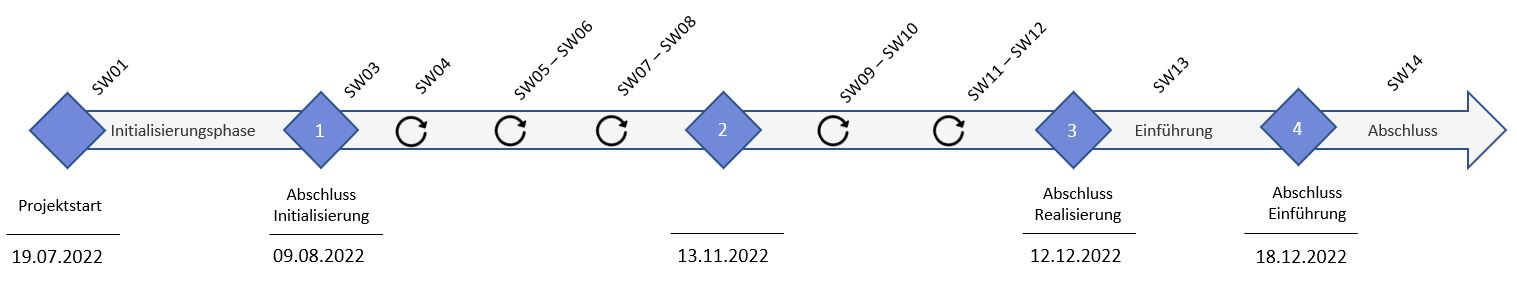
\includegraphics[width=1.3\textwidth]{img/Rahmenplan.jpg}
    \caption{Rahmenplan}
    \label{fig:Rahmenplan}
\end{figure}
\todo{Hinzufügen von Meilenstein am Anfang von Projekt}
\todo{Datum bei Projektstart stimmt nicht}
Es wurde entschieden eine Intialisierungsphase von 3 Wochen zu planen, da die Analyse der bestehenden Software in dieser Phase stattfindet.
Am Schluss bleibt noch eine Woche für die Einführungsphase und das Erstellen der Anleitung.
Für die Realisierungsphase bleiben 9 Wochen Zeit, die in Sprints eingeteilt werden können.
Es verbleibt ein einwöchiger Sprint und 4 reguläre zweiwöchige Sprints.

\subsubsection*{Meilensteine}
Meilensteine erlauben es den Projektfortschritt festzustellen,
in dem zuvor definierte Projektergebnisse (Artefakte) an einem gewissen Datum vorliegen.\\
Artefakte sind konkrete Dokumente oder Software die vorliegen muss. Zum Beispiel:
\begin{itemize}
    \item Testprotokolle
    \item Prototypen
    \item Software Releases
    \item Sprintplannungen
    \item etc.
\end{itemize}

In SoDa ist es normal, bei jedem Phasenwechsel ein Meilenstein zu definieren und in der Mitte der
Realisierungsphase noch einmal. \autocite{jenny_projektmanagement_2016} % PMB Projektplanung p23-25
Nach diesem Vorgehen erhält man 5 Meilensteine für dieses Projekt.

\begin{table}[h]
    \centering
    \begin{tabular}{|l|l|l|}
        \hline
        \rowcolor[gray]{.9} MS & Datum & Artefakte \\
        \hline
        1 & 19.09.2022 & \tabitem Aufgabenstellung \\
        \hline
        2 & 09.10.2022 & \tabitem Architekturdokument \\
         & & \tabitem Analyse \\
         & & \tabitem Testkonzept \\
         & & \tabitem Sprintplannung 1 \\
        \hline
        3 & 13.11.2022 & \tabitem Software-Release 0.5 \\
         & & \tabitem Sprintplannung 4 \\
        \hline
        4 & 12.12.2022 & \tabitem Software-Release 1.0 \\
         & & \tabitem Dokumentation Realisierung \\
        \hline
        5 & 18.12.2022 & \tabitem Bedienungsanleitung \\
        \hline
    \end{tabular}
    \caption{Meilensteine}
    \label{tab: Meilensteine}
\end{table}

\subsection{Anforderungen}
Aus dem Projektauftrag und aus den Wünschen der Stakeholder werden Anforderungen an das Produkt definiert.
Diese werden für die Realisierungsphase in Epics umgewandelt.
Die Epics werden im Anschluss in einzelne User Stories aufgeteilt, die dann in den Sprints seperat behandelt und gelöst werden.
\newpage

\subsubsection{Epics}\label{Epics}
Für das Projekt werden folgende Epics definiert.

\begin{table}[h]
    \centering
    \begin{tabular}{ | p{1em} | p{35em} | p{2em} |}
        \hline
        \rowcolor[gray]{.9} ID & Beschreibung & Prio \\
        \hline
        1 & Der Nutzer wird beim erstmaligen Betreten des Discord-Servers vom Bot benachrichtigt.
        Dieser gibt ihm Grundlegende Informationen zum Server und dem Authentisierungsprozess.
        Zu diesem Zeitpunkt hat der Student noch keine Berechtigungen auf dem Server und
        hat nur Zugriff auf den Channel "Help". & A \\
        \hline
        2 & Der Bot soll den Nutzer authentifizieren und mit der Studenten-Rolle versehen können.
        Er kann dabei zwischen den E-Mails von Nicht-Student und Student unterscheiden und auf unvorhergesehene
        Interaktionen, von Seiten des Benutzers, reagieren können. & A \\
        \hline
        3 & Ein Student kann sich beim Bot für ein Modul anmelden. Dieser schaltet den Channel für den Studenten frei,
        so das er darin mit anderen Studierenden kommunizieren kann. Falls das Modul für den Studenten nicht mehr relevant ist,
        kann er es beim Bot wieder abmelden. & A \\
        \hline
        4 & Die Administration des Discord Servers soll einfach neue Modullisten in das System laden können.
        Die neuen oder nicht mehr Verfügbaren Module werden erkannt und entsprechend hinzugefügt oder gelöscht.
        An dem Verhalten des Benutzers soll sich nichts ändern. & A \\
        \hline
        5 & Die Adminsitration kann jedes Semster die neuen Studierenden hinzufügen.
        Diese werden beim potentiellen Authentifizieren direkt in Ihre zugeteilten Häuser-Channels zugewiesen. & A \\
        \hline
        6 & Die Administration von Stair kann über eine zur Verfügung gestellte Schnittstelle Statistiken über
        den Discord erstellen können. & B \\
        \hline
        7 & Fehlereingaben in den Modulregistrierungschannel oder interne Fehler vom Bot, sollen direkt automatisch
        an einen hinterlegten Mitarbeiter von Stair gemeldet werden & C \\
        \hline
    \end{tabular}
    \caption{Epics}
    \label{tab: Epics}
\end{table}

\subsubsection{User Stories}
Die Epics werden in kleinere User-Stories heruntergebrochen und dienen als Bausteine eines Sprints.
Dieser Prozess wird auch \textbf{Story-Splitting} genannt
User-Stories sind immer nach dem gleichen Muster aufgebaut. \\
"Als <Rolle> möchte ich <Ziel/Wunsch>, um <Nutzen>." \\
Die Story muss nicht immer aus der Benutzersicht definiert sein, sondern es können auch technische oder 
infrastrukturelle User-Stories so gebildet werden.

In der Strintplannung werden zu jeder User-Story zugehörige Akzeptanzkriterien definiert.
Diese dienen zur Kontrolle, ob die User-Story korrekt umgesetzt wurde und 
können auch als Test während der Entwicklung gebraucht werden.
Später können dann die Mitglieder des Teams, den Aufwand der Story realistisch abschätzen.

Gute User-Stories können nach dem Modell \textbf{I.N.V.E.S.T} gebildet werden. \autocite{hammerschall_software_2013} % PMB Projektplanung p.101-103
\begin{itemize}
    \item \textbf{I}ndependent  unabhängig voneinander
    \item \textbf{N}egotiable   zerlegbar, änderbar, kombinierbar, verhandelbar
    \item \textbf{V}aluable     hat wirtschaftlichen Wert
    \item \textbf{E}stimatable  so klar, dass es vom Team geschätzt werden kann
    \item \textbf{S}mall        klein genug, um in einem Sprint entwicklet werden zu können
    \item \textbf{T}estable     klare Akzeptanzkriterien
\end{itemize}

Beim Story-Splitting werden folgende User-Stories für das Projekt definiert. 

\begin{longtable}{ | p{1em} | p{16em} | p{13em} | p{2em} | p{3em} | p{2em} |}
    \hline
    \rowcolor[gray]{.9} ID & Beschreibung & Akzeptanzkriterien & Prio & Weight & Sprint \\
    \hline
    1 & Als Bot möchte ich den Benutzer beim ersten Betreten des Server authentifizieren können,
    um ihm die ihm zugeteilten Rollen zuweisen zu können. & 
    \tabitem Der Nutzer bekommt beim ersten Betreten des Servers eine Nachricht vom Bot mit Informationen. & A & 12 & 2 \\*
    & & \tabitem Der Student bekommt nach der Anmeldung die Rolle Student zugeteilt und wird dem richtigen Haus-Channel zugewiesen. & & & \\
    \hline
    2 & Als Bot möchte ich den Studenten mittels E-Mail Verifikation authentifizieren können,
    um sicher zu gehen, dass dieser eine gültige Studenten-Mail besitzt. &
    \tabitem Der Student bekommt eine E-Mail auf der Adresse, die er dem Bot mitteilt. & A & 15 & 3 \\*
     & & \tabitem Ein Student kann sich authentifizieren, ein Nicht-Student wird abgewiesen. & & & \\*
     & & \tabitem In der E-Mail steht ein zufällig generierter 6-stelliger Code. & & & \\*
     & & \tabitem Der Bot kann den Code verifizieren, nachdem der Student die E-Mail erhalten hat. & & & \\
    \hline
    3 & Als Stair Administrator möchte ich neue Studenten einfach erfassen können,
    um sie dem System bekannt zu machen und die Administration zu vereinfachen. & 
    \tabitem Neue Studenten können mit ihren zugeteilten Häusern als Liste eingelesen werden & B & 9 & 1 \\*
     & & \tabitem Die neu erfassten Studenten werden im System eingetragen und können für die Authentifizierung verwendet werden. & & & \\
    \hline
    4 & Als Student möchte ich mich für neue Modul-Channels an und abmelden können,
    um mich mit anderen Studenten austauschen zu können. & 
    \tabitem Es stehen Befehle im \textbf{Registrierungs-Channel} zur Verfügung, um sich bei Modulen an- und abzumelden. & A & 12 & 3 \\*
     & & \tabitem Der Bot weist den Studenten, bei einer Anmeldung, dem Modul als Mitglied hinzu. & & & \\*
     & & \tabitem Der Bot löscht den Studenten, bei einer Abmeldung, aus der Mitgliederliste, 
     so dass der Channel für den Studenten nicht mehr sichtbar ist. & & & \\ 
    \hline
    5 & Als Stair Administrator möchte ich Modullisten mit den verfügbaren Modulen, einfach in das System eintragen zu können,
    um sie für den Bot nutzbar zu machen. &
    \tabitem Pro Semester können Modullisten automatisch eingelesen werden. & B & 12 & 2 \\*
     & & \tabitem Neue Module werden automatisch hinzugefügt, und solche, welche nicht mehr Unterrichtet werden, werden gelöscht. & & & \\*
     & & \tabitem Die Module stehen nach dem einlesen direkt bereit, zur Channel-Erstellung durch den Bot. & & & \\
    \hline
    6 & Als Stair Administrator möchte ich Statistiken aus dem System auslesen können,
    um sie für Marketing oder andere Zwecke gebrauchen zu können. & 
    \tabitem Es stehen ein paar vorgefertigte Auslesemöglichkeiten bereit, um sie für den Administrator nutzbar zu machen & C & 9 & 4 \\
    \hline
    7 & Als Stair Administrator möchte ich sofort benachrichtigt werden, falls mit dem System ewtwas nicht stimmt,
    um Gegenmassnahmen ergreifen zu können. & 
    \tabitem Der Administrator wird benachrichtigt, wenn der Bot zu Discord oder zur Datenbank keine Verbindung mehr hat & C & 5 & 5 \\*
     & & \tabitem Der Administrator wird benachrichtigt wenn der E-Mail Versand zur Authentifikation nicht mehr funktioniert. & & & \\
    \hline
    \caption{User-Stories}
    \label{tab: UserStories}
\end{longtable}
\clearpage
\subsubsection*{Sprintplanung}
\begin{table}[h]
    \centering
    \begin{tabular}{|l|l|l|l|}
        \hline
        \rowcolor[gray]{.9} Sprint & Start & Ende & Artefakte \\
        \hline
        Sprint 1 & 10.10.2022 & 16.10.2022 & \tabitem Studentenerfassung implementiert \\
         & & & \tabitem Sprintreview S01 \\
         & & & \tabitem Sprintplannung S02 \\
        \hline
        Sprint 2 & 17.10.2022 & 30.10.2022 & \tabitem Modulerfassung implementiert \\
         & & & \tabitem Sprintreview S02 \\
         & & & \tabitem Sprintplannung S03 \\
        \hline
        Sprint 3 & 31.10.2022 & 13.11.2022 & \tabitem Authentifizierung implementiert \\
         & & & \tabitem Sprintreview S03 \\
         & & & \tabitem Sprintplannung S04 \\
        \hline
        Sprint 4 & 14.11.2022 & 27.11.2022 & \tabitem Statistiken implementiert \\
         & & & \tabitem Sprintreview S04 \\
         & & & \tabitem Sprintplannung S05 \\
        \hline
        Sprint 5 & 28.11.2022 & 11.12.2022 & \tabitem Fehlererkennung implementiert \\
         & & & \tabitem Sprintreview S05 \\
        \hline
    \end{tabular}
    \caption{Sprintplanung}
    \label{tab: Sprintplanung}
\end{table}

Die Projektkontrolle und der Fortschritt wird mit folgenden Tools überwacht.
\begin{itemize}
    \item Github Story-Board (\href{https://github.com/orgs/stairch/projects/1/views/4}{Link zum Story-Board})
    \item Sprintreviews (\nameref{Sprintreviews})
\end{itemize}

\subsection{Risikomanagement}
Risikomanagement

\newpage
\section{Realisierung}

\subsection{Analyse der bestehenden Infrastruktur}
Als erster Schritt wird eine Analyse des bestehenden Bots und seiner Funktion im Discord durchgef\"uhrt.

\subsubsection{Aufbau Discord}
Der Discord Server "Stair" wird von Stair verwaltet und ist ein online Treffpunkt f\"ur alle Studenten des Departements Informatik.
Beim erstmaligen Eintretten in den Server hat man noch keine Berechtigung und es wird deshalb noch nichts, ausser dem Help Channel
angezeigt. Man bekommt vom Bot Stan, beim Eintretten auf den Server, eine Nachricht mit einer Anleitung. Darin ist beschrieben, wie
man sich authentifizieren kann. Bei der Authentifizierung wird vom Bot geschaut ob es sich um eine Studenten E-Mail Adresse handelt.
Wenn dem so ist, schickt der Bot einen 6-stelligen Random Code, den der Benutzer im Discord dem Bot zur\"uckschreiben muss.

Hat dieser Prozess funktioniert, ist man "eingeloggt" und bekommt vom Bot die Rolle Student zugeteilt. Damit hat man Zugriff auf
die verschiedenen Grundchannels, wie Gaming, Administration, General, Studying, etc.
In diesen Channels kann man sich mit seinen Mitstudierenden Sprachlich oder per Text \"uber alle Themen austauschen.
\newline

Der Stair Discord-Server bietet auch Informationen und Unterst\"utzung f\"ur alle Module an. Dabei hat jedes Modul einen eigenen Channel.
Dort k\"onnen sich Studierende gezielt \"uber ein Modul austauschen, Fragen stellen oder Informationen mitteilen.
Am Anfang wird gar nichts angezeigt. Man muss sich spezifisch f\"ur die Module registrieren um diese angezeigt zu bekommen. Dies verhindert

\begin{enumerate}
    \item dass man unn\"otig Benachrichtigungen von Channels bekommt, die einen nicht interessieren.
    \item dass sein Discord nicht \"uberf\"ullt wird mit 400 Modul-Channels.
\end{enumerate}

Die Commands \textit{show <module>} und \textit{hide <module>} erlauben es, den Channel hinzuzuf\"ugen oder zu entfernen.
\newline

Neu gibt es auch das Konzept von verschiedenen H\"ausern bei Stair. Jeder Student wird dabei einem Haus zugeteilt. Die Zuteilung l\"auft
dabei \"uber das Sekretariat der Hochschule. Es wird geschaut, dass in jedem Studiengang in jedem Startsemester, die Studenten gleichm\"assig
auf die H\"auser verteilt werden.
Es gibt die H\"auser Blue, Purple, Red, Orange, Yellow und Grey. \"uber das Semester hinweg organisiert Stair verschiedene Events, bei denen
man Punkte f\"ur sein Haus sammeln kann. Am Ende jedes Jahres, also Ende Fr\"uhlingssemster, wird das Haus, welches am meisten Punkte
gesammelt hat, als Gewinner gelobt.

Der Discord-Server bietet die Platform um sein Haus zu mobilisieren oder die neuesten Ergebnisse den Studenten zu verk\"unden.
Pro Haus gibt einen Channel. Momentan werden die Studenten noch manuell zu ihren zugeh\"origen Channels hinzugef\"ugt.
\newline
\newline
\todo{Bild von Discord und Channels anzeigen}

\subsubsection*{Ablauf Athentifizierung}
\todo{Nicolas}
\todo{Bild Ablaufdiagramm Authentifizierung}


\subsubsection*{Ablauf Modul-Channel Einschreibung}
\todo{Bild Ablaufdiagramm Modul}


\subsubsection{Funktionsweise Bot}
Der Bot ist mit der Programmiersprache C\# und dem .NET Framework geschrieben.

\subsubsection*{Konfigurationsmanagement alter Bot}
In der folgenden Tabelle ist eine \"Ubersicht der benutzen IDE, ihrer Spezifizierung und den eingesetzten Libraries.
\todo{Tabelle mit Spezifikationen vom System. (Versionen, Libraries)}
\newline


Das Programm, welches den Bot zur Verfügung stellt, ist nicht gross. Es beinhaltet im Groben einen Client Socket der
Events on Discord abfängt und einer E-Mail Klasse, die E-Mails an den Benutzer versenden kann.
Das Programm ist in zwei Packages aufgeteilt.

\begin{itemize}
    \item StanBot.Core
    \item StanBot.Service
\end{itemize}

\todo{Bild Klassendiagramm Bot}

\subsubsection{Ausführung Bot}

Der Bot läuft auf einem Windows Server \#\#\#\# auf der Enterprise Lab Umgebung der HSLU. Die Konfiguration entspricht der eines
Windows Services und läuft dementsprechend durchgehend.
\newline
\todo{Bild Service Konfiguration}
\newline


\subsubsection{Geplante Änderungen}
\todo{Yannis}

\subsubsection*{Wechsel zu Linux Server}

Es wurde zusammen mit dem STAIR Team entschieden,
auf Linux zu wechseln um alle Server einheitlich auf Linux zu haben.
\todo{Wordpress erklären}
Bei STAIR wird noch eine Wordpress-Seite und eine JavaScript Webseite betrieben.
Da die Projekte jedoch sich von einander stark unterscheiden wurde entschieden mit verschiedenen Servern zu arbeiten und nicht alle auf dem gleichen Server zu hosten.

\subsubsection*{Entscheid den Bot neu zu schreiben}

\todo{replace .NET Standard with .NET Framework version}
\todo{Add sources}
Bei der Analyse des bisherigen Bot wurde bemerkt, dass die veraltete Technologie .NET Standard 2.0 und .NET Core mit 3.1 mit veralteten Libraries genützt wurden.
Diese werden nicht mehr unterstützt und sollten ersetzt werden.
Hierbei wird .NET 6 mit C# verwendet.
So kann man Teile des Codes wiederverwenden.
Die neueren .NET Versionen sind Cross-Platform fähig und können damit nun auch auf Linux verwendet werden. \todo{source}
Die Sprache wird nicht an der Hochschule breit verwendet, es gibt jedoch ein Modul dazu und ist ähnlich zu Java,
welche grundsätzlich an der Hochschule verwendet wird. \todo{source}

\todo{ist "wir" okay hier?}
Aus persönlicher Erfahrung finden wir, dass Java häufiger zu Problemen führt als C#.

\subsubsection*{Entscheid Login Funktionsweise}
\todo{source}
Beim Login wurde überlegt das Switch-Login der Hochschule zu verwenden, welches auch für aussenstehende Zwecke verwendet werden kann.
Hierbei wurde dagegen entschieden, da STAIR nicht die volle Kontrolle über den Service hat und deshalb plötzlich neue Interface Standards erlassen werden können, was zu Problemen führen kann.
Auch muss hierzu ein bestimmter Link geöffnet werden, welcher von Stan verschickt werden muss um die Switch Login Seite zu öffnen.
Dies könnte nicht vertrauenswürdig wirken bei Studenten.
Ausserdem hat sich das Login mittels E-Mails bereits bewährt, weshalb dieses nun weiterhin verwendet wird.

\subsubsection*{Wechsel zu Community Server}

Entscheid Anbindung an Datenbank
- Einfachere Verwaltung von Studenten und Modulen
- Einfachere Kontrolle und Steuerung von Stair
- Erweiterbarkeit und Weeiterentwicklung
- Anbindung von anderen Tools/Programmen an Datenbank (Statistik/Zukunft)

Entscheid schreiben eines eigenen Bots
- Bestehender Bot
- Datenschutz
- Kontrolle und Handlungsspielraum
- Statistiken
- Keine ungewollten Features

\newpage
\section{Evaluation und Validation}

\todo{schreiben}

\subsection{Fehlererkennung}

\section{Ausblick}

\todo{schreiben}

\newpage

\section{Anh\"ange}

\subsection{Sprintreviews}\label{Sprintreviews}
In diesem Kapitel werden die einzelnen Sprintreviews augelistet.
Diese beinhalten immer eine Reflektion zum letzten Sprint mit einer Übersicht der umgesetzten User-Stories und 
einer Retrospektive über aufgefallenen Problemen und dazugehörigen Massnahmen.

\subsubsection{Sprint 1}
\subsubsection*{Sprintziel}
Ziel

\subsubsection*{Risiko-Update}
Update

\subsubsection*{Sprintbacklog}
Link zu dem Backlog für den Sprint 1:\\
% Link
Aufwandschätzung für den Sprint: XX Story Points

\subsubsection*{Sprintreview}
Bild von Burndown-Chart

Geschätzter Aufwand: XX \\
Effektiver Aufwand: XX \\

Bild von Umgesetzten User Stories aus dem Backlog.

\subsubsection*{Retrospektive}
Erfolge:
\begin{itemize}
    \item XX 
\end{itemize}
Probleme:
\begin{itemize}
    \item XX
\end{itemize}
Massnahmen:
\begin{itemize}
    \item XX 
\end{itemize}

\subsubsection{Sprint 2}
Same for Sprint 2
\newpage

\section{Glossar}

% https://blog.aristolo.com/de/definition-begriffe-bachelorarbeit-masterarbeit-dissertation/
\todo{schreiben}

\section{Abbildungsverzeichnis}
\listoffigures

\section{Tabellenverzeichnis}
\listoftables

\section{Literaturverzeichnis}
\printbibliography

\end{document}
